% !TEX encoding = UTF-8 Unicode
\documentclass{article}
\usepackage{superstyle}
\begin{document}



Forside
\newpage


\section{Forord} % (fold)
\label{sec:forord}
Denne rapporten er resultatet av et prosjekt ved dataingeniørlinjen på HiST. Oppgaven har blitt utført vårsemesteret 2015. 
\vspace{5mm}


I vårt arbeid med denne oppgaven har vi benyttet oss av mange teknologier som har forenklet prosessen betraktelig, eksempelvis og spesielt Latex, Github, Google Docs, MatLab og Sublime har alle vært til stor hjelp får å produsere det endelige resultatet. 
\vspace{5mm}

Vi vil også takke Hans Jakob Rivertz for god veiledning gjennom hele prosjektet. 

\newpage
% section forord (end)



\section{Sammendrag} % (fold)
\label{sec:sammendrag}
Denne rapporten omhandler Euler-Bernoulli bjelken (The Euler-Bernoulli beam). Dette er en fundamental modell som sier hvordan forskjellige materialer bøyer seg under påvirkning av diverse krefter. Modellens nøyaktighet ble praktisk demonstrert da den ble brukt til å bygge både Eiffel-tårnet og Pariserhjulet \cite{NdogmoEB}.  Det viser seg at diskretisering av differentialligningen gjør at vi får et system av lineære ligninger som kan brukes til å finne den vertikale forskyvningen. Jo mindre steglengde vi bruker til diskretiseringen, jo større blir likningssystemet. Euler-Bernoulli modellen er en meget sentral modell innenfor dette området, og det er skrevet mange artikler rundt dette. \\

I rapporten går vi først igjennom grunnleggende teori som utgjør grunnlaget for utregningene gjort for å regne ut den vertikale forskyvningen i hvert punkt langs bjelken. På grunn av at oppgaven vi har fått er en faktisk oppgave som står i læreboken [KILDE HER KANSKJE?! :D ], går vi i teoridelen igjennom de fleste formlene boken oppgir, med noen få unntak som spesifikt ikke skulle beskrives. Til slutt i teoridelen følger det 2 bevis. Det ene beviset beviser likning 2.28, som er et uttrykk på den fjerdederiverte til funksjonen y i Euler-Bernoulli likningen. Av grunner beskrevet i teoridelen er ikke denne likningen brukbar langs hele planken, og derfor følger et nytt bevis på den fjerdederiverte i punktet $x_1$ etter dette. \\

Etter teoridelen løser vi en rekke oppgaver. Oppgavene vi løser er oppgavene som står til slutt i Reality Check 2 (HVORDAN SIER MAN DETTE?!), og går ut på forskjellige utregninger knyttet til et stupebrett, som enkelt kan relateres til Euler-Bernoulli-likningen. Oppgavene går fra å lage diverse MatLab-programmer som regner ut den vertikale forskyvningen langs planken, på forskjellige måter, til både det å finne hvor store feil forskjellige funksjoner har. Vi får også oppgitt en løsning på funksjonen, som vi skal vise at tilfredsstiller Euler-Bernoulli funksjonen, gitt en viss påført kraft. Til slutt regner vi også den vertikale forskyvningen når vi påfører vekt på stupebrettet. \\ 

NOEN VIKTIGE RESULTATER? :D 

KILDER: 

http://arxiv.org/pdf/1110.6029.pdf - EIFFEL TOWER :D :D :D 
\newpage
% section sammendrag (end)


%\section{Innholdsfortegnelse og figur- og tabelliste} % (fold)
\label{sec:innholdsfortegnelse_og_figur_og_tabelliste}
\renewcommand{\contentsname}{Innholdsfortegnelse og figur- og tabelliste}
\tableofcontents
\newpage
% section innholdsfortegnelse_og_figur_og_tabelliste (end)



\section{Teori og metode} % (fold)
\label{sec:teori}
Denne delen kan variere litt fra oppgave til oppgave. Vanligvis vil den inneholde en beskrivelse av hva som er gjort hittil pa fagfeltet man arbeider med, samt annen bakgrunnsinformasjon som er nødvendig for a forsta det arbeidet som utføres i oppgaven. En del ingeniøroppgaver vil ogsa kunne benytte matematikk (og av og til fysikk) som det ikke kan forventes at leseren skal ha intimkunnskap om pa forhand. Denne vil da beskrives her. For en studentoppgave bør det i et slikt tilfelle alltid redegjøres for all matematikk og fysikk som eventuelt benyttes.


Vi skal i denne oppgaven jobbe mye med Euler-Bernoulli modellen for materialers bøyning under påvirkning av krefter. Modellen yttrykker den vertikale forskyvningen f(x) hvor $0\leq x \leq L$. x går langs bjelken som har lengde L. Euler-Bornoulli likningen er gitt ved 
\begin{align}
    EIy''''=f(x)
\end{align}
hvor E er Youngs modulus til materialet, og I er tregheten. Begge disse er konstante langs hele bjelken. Funksjonen f(x) er er den påførte kraften, inkludert bjelkens egenvekt, per lengde-enhet. 
\\ \\
I oppgaven (Reality Check 2) har vi oppgitt formelen 2.27 og 2.28 som følger (et bevis på 2.28 kommer senere): 
\begin{align}
    EIy''''&=f(x) \nonumber \\
    y''''(x)& \approx \frac{y(x-2h)-4y(x-h)+6y(x)-4y(x+h)+y(x+2h)}{h^4}
\end{align}
Vi deler opp planken i $n$ like deler, alle med lengde $h=\frac{L}{n}$. Dette medfører at $x_0<x_1<x_2...<x_i$, hvor alle $x_i$ har lengde $h$. $x_0$ er starten på planken, $x_1$ er første steglengde ut på bjelken, $x_1=1\cdot h$. $x_2$ er på samme måte andre lengde ut på planken, $x_2=2\cdot h$. Videre blir $x_i=i\cdot h$. Hvis vi sier at $y_i=y(x_i)$ og setter dette inn i likning 2.27 får vi at 

\begin{align}
EI\cdot	\frac{y_{i-2}-4y_{i-1}+6y_i-4y_{i+1}+y_{i+2}}{h^4}=f(x)
\end{align}
Vi gjør om slik at vi får alle leddene som inneholder y på én side:
\begin{align}
    y_{i-2}-4y_{i-1}+6y_i-4y_{i+1}+y_{i+2}=\frac{h^4}{EI}f(x_i)
\end{align}
Dette er hvordan man kommer frem til likning 2.29. 
\\ \\ 
Videre skal vi bruke Euler-Bernoulli likningen på et stupebrett. Et stupebrett er en bjelke som er festet i den ene enden, og den vertikale forskyvningen på starten av brettet er naturligvis lik 0. Hvis vi bruker dette får vi følgende informasjon om starten av brettet ($y(0)$) og slutten av brettet ($y(L)$):
\begin{align}
    y(0)=y'(0)=y''(L)=y'''(L)=0
\end{align}
Men, skal vi bruke de tidligere definerte funksjonene får vi et problem. Vi ser at hvis vi har lyst til å finne den vertikale forskyvningen i det første punktet etter starten, altså $x_1$, blir dette umulig. Som sagt tidligere er $x_1=1\cdot h$, og setter vi dette inn i formelen vi tidligere har definert for den fjerdederiverte får vi: 

\begin{align}
	y''''(x_1)&\approx \frac{y((1\cdot h)-2h)-4y((1\cdot h)-h)+6y(1\cdot h)-4y((1\cdot h)+h)+y((1\cdot h)+2h)}{h^4}\nonumber \\
	y''''(x_1)&\approx \frac{y(-h)-4y(0)+6y(h)-4y(2h)+y(3h)}{h^4}
\end{align}
Bruker notasjonen $y_i=y(x_i)$, hvor $x_i$ er som før, får vi at: 

\begin{align}
    y_{-1}-4y_0+6y_1-4y_2+y_3&=\frac{h^4}{EI}f(x_1)
\end{align}
Det er her vi har et problem. $y_{-1}$ er ikke definert grunnet at vi har ingen punkter som kommer før stupebrettets begynnelse. Derfor trenger vi et nytt uttrykk for $y''''(x)$ som gjelder bare for $x_1=1 \cdot h$. Dette uttrykket er som følger (bevis kommer senere) : 

\begin{align}
    y''''(x_1) &\approx \frac{16y(x_1)-9y(x_1+h)+\frac{8}{3}y(x_1+2h)-\frac{1}{4}y(x_1+3h)}{h^4}
\end{align}

Vi har altså et generelt uttrykk for $y''''(x)$, med et unntak for $y(x_1)$. Dette er, som sagt før: 
\begin{align}
     y''''(x)& \approx \frac{y(x-2h)-4y(x-h)+6y(x)-4y(x+h)+y(x+2h)}{h^4}
 \end{align} 
 Som vi ser av dette uttrykket bruker det punktene $x+h$ og $x+2h$. Vi har altså litt av det samme problemet som vi hadde for $x_1$: På slutten av planken, ved $x=L$, vil uttrykket inneholde punktene $L+h$ og $L+2h$. Vi har altså 2 punkter som er lengre enn brettets lengde, og derfor trenger vi nye uttrykk for $y''''(x_{n-1})$ og $y''''(x_n)$. Disse er som følger (skal ikke bevises, antas som gyldige): 
\begin{align}
    y''''(x_{n-1})&\approx \frac{-28y_n+72y_{n-1}-60y_{n-2}+16y_{n-3}}{17h^4} \\
    y''''(x_n)&\approx \frac{72y_n-156y_{n-1}+96y_{n-2}-12y_{n-3}}{17h^4}
\end{align}

Vi har nå gyldige uttrykk for hele plankens lengde. I bokas likning/figur 2.34 er matrisen som avbildet i figur \ref{fig:EBMatrix}. 
\begin{figure}[h]
    \centering
    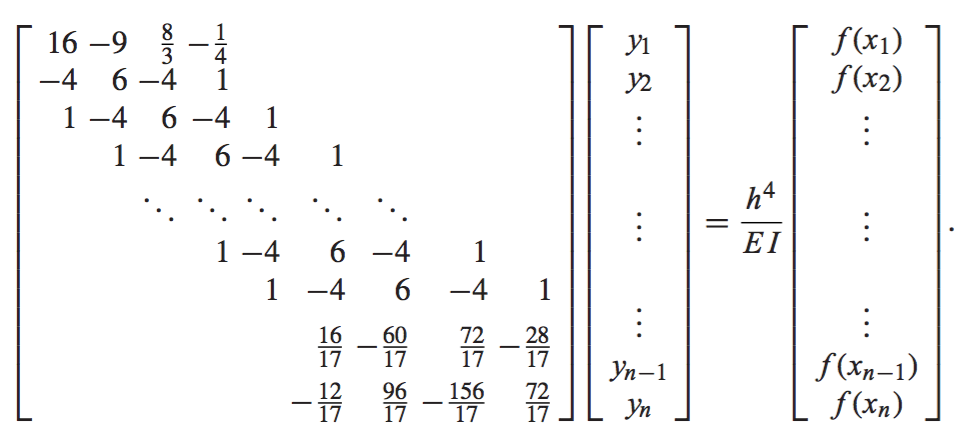
\includegraphics[width=0.8\textwidth]{sections/Theory/EBMatrix}
    % \includegraphics[width=0.8\textwidth]{errorplot2}
    \caption{Matrisen 2.34 fra boken}
    \label{fig:EBMatrix}
\end{figure}
Tallene i denne matrisen stemmer godt med likningene vi har funnet. Likningen for $x_1$ hadde koeffisientene 16, -9, $\frac{8}{3}$ og $-\frac{1}{4}$, og dette stemmer overens med første linje i matrisen. Resten av matrisen, frem til de 2 siste leddene, skulle ha koeffisientene 1, -4, 6, -4 og 1. Linje 2, altså $x_2$, har koeffisientene -4, 6, -4 og 1. Dette er fordi det generelle uttrykket er 

\begin{align}
    y''''(x)& \approx \frac{y(x-2h)-4y(x-h)+6y(x)-4y(x+h)+y(x+2h)}{h^4} \nonumber
\end{align}
og i $x=2h$ er $y((2\cdot h)-2h)=y(0)=0$. De 2 siste linjene i matrisen stemmer overens med uttrykkene vi fant for $y''''(x_{n-1})$ og $y''''(x_n)$. 
\\ \\
Følgende kommer et bevis på at den fjerdederiverte (likning 2.28) kan approksimeres ved: 

\begin{align}
    f^{iv}(x)=\frac{f(x-2h)-4f(x-h)+6f(x)-4f(x+h)+f(x+2h)}{h^4}\nonumber
\end{align}

Først setter vi opp taylor-rekker for punktene $x+2h$, $x-2h$, $x+h$, $x-h$: 
\begin{align}
    f(x+2h)&=f(x)+2hf'(x)+2h^2f''(x)+\frac{(4h)^3}{3!}f'''(x)+\frac{(2h)^4}{4!}f^{(4)}(x)+\frac{(2h)^5}{5!}f^{(5)}(x)+h^6\nonumber\\ 
    f(x-2h)&=f(x)-2hf'(x)+2h^2f''(x)-\frac{(4h)^3}{3!}f'''(x)+\frac{(2h)^4}{4!}f^{(4)}(x)-\frac{(2h)^5}{5!}f^{(5)}(x)+h^6\nonumber\\
    f(x+h)&=f(x)+hf'(x)+\frac{h^2f''(x)}{2}+\frac{h^3}{3!}f'''(x)+\frac{h^4}{4!}f^{(4)}(x)+\frac{h^5}{5!}f^{(5)}(x)+h^6\nonumber\\
    f(x-h)&=f(x)-hf'(x)+\frac{h^2f''(x)}{2}-\frac{h^3}{3!}f'''(x)+\frac{h^4}{4!}f^{(4)}(x)-\frac{h^5}{5!}f^{(5)}(x)+h^6\nonumber
\end{align}

Deretter legger vi først sammen $f(x+2h)$ og $f(x-2h)$: 

\begin{multline}
    \\
    f(x+2h)+f(x-2h)= \\
    f(x)+2hf'(x)+2h^2f''(x)+\frac{(4h)^3}{3!}f^3(x)+\frac{(2h)^4}{4!}f^{4}(x)+\frac{(2h)^5}{5!}f^{(5)}(x)+h^6 \\
    + \\
  	f(x)-2hf'(x)+2h^2f''(x)-\frac{(4h)^3}{3!}f^3(x)+\frac{(2h)^4}{4!}f^{4}(x)-\frac{(2h)^5}{5!}f^{(5)}(x)+h^6\nonumber \\
  	=\\
  	2f(x)+4h^2f''(x)+\frac{4}{3}h^4f^{(4)}(x)+h^6 \nonumber\\
\end{multline}

Deretter legger vi sammen $f(x+h)$ og $f(x-h)$: 
\begin{multline}
	f(x)+hf'(x)+\frac{h^2f''(x)}{2}+\frac{h^3}{3!}f'''(x)+\frac{h^4}{4!}f^{(4)}(x)+\frac{h^5}{5!}f^{(5)}(x)+h^6\\
	+\\
	f(x)-hf'(x)+\frac{h^2f''(x)}{2}-\frac{h^3}{3!}f'''(x)+\frac{h^4}{4!}f^{(4)}(x)-\frac{h^5}{5!}f^{(5)}(x)+h^6\\
	=\\
	2f(x)+h^2f''(x)+\frac{h^4f^{(4)}(x)}{12} + h^6 \nonumber \\
\end{multline}

Til slutt legger vi sammen $f(x+h)+f(x-h)$ og $\frac{f(x+2h)+f(x-2h)}{4}$: 
\begin{multline}
	\\
	2f(x)+h^2f''(x)+\frac{h^4f^{(4)}(x)}{12} + h^6 \\
	+\\
	\frac{2f(x)+4h^2f''(x)+\frac{4}{3}h^4f^{(4)}(x)+h^6 }{4}\\
	=\\
	\frac{3}{2}f(x)-\frac{3}{12}h^4f^{(4)}(x)+h^6
\end{multline}

Deretter løser vi likningen med hensyn på $f^{(4)}(x)$: 
\begin{align}
    f(x+h)+f(x-h)-\frac{f(x+2h)}{4}-\frac{f(x-2h)}{4}=\frac{3}{2}f(x)-\frac{3}{12}h^4f^{(4)}(x)+h^6\nonumber
\end{align}
\begin{align}
     -3h^4f^{(4)}(x)&=12f(x+h)+12f(x-h)-3f(x+2h)-3f(x-2h)-18f(x) +h^6 \nonumber \\
     \nonumber \\
	f^{(4)}(x)&=\frac{-4f(x-h)+f(x-2h)+6f(x)+f(x+2h)-4f(x+h)}{h^4}
\end{align}
 

Her kommer det andre beviset: 
\begin{align}
f(x+2h)+f(x-2h)+f(x+h)+f(x-h)=f4(x)+5h^2f''(x)+\frac{17}{12}h^{(4)}(x)+h^6 \nonumber
\end{align}

Vi setter $f^{(4)}$ alene, og får: 

\begin{align}
	f^{(4)}=\frac{12f(x+2h)}{17h^4}+\frac{12f(x-2h)}{17h^4}+\frac{12f(x+h)}{17h^4}+\frac{12f(x-h)}{17h^4}-\frac{48f(x)}{17h^4}-\frac{60f''(x)}{17h^2}+\frac{h^6}{h^4}
\end{align}

Vi ser at vi trenger $f''(x)$. HER SKAL VI FINNE DEN; HVORDAN GJØR VI DET?!??!?!?! 
Setter vi dette inn i uttrykket vi har for $f^{(4)}(x)$ får vi: 

\begin{multline}
    f^{(4)}(x)=\frac{12f(x+2h)}{17h^4}+\frac{12f(x-2h)}{17h^4}+\frac{12f(x+h)}{17h^4}+\frac{12f(x-h)}{17h^4}-\frac{48f(x)}{17h^4}-\\ \frac{60f}{17h^2}\cdot (\frac{-f(x+2h)+16f(x+h)-30f(x)+16f(x-h)-f(x-h)}{12h^2})+\frac{h^6}{h^4} \nonumber
\end{multline}

\begin{multline}
    f^{(4)}(x)=\frac{12f(x+2h)}{h^4}+\frac{12f(x-2h)}{h^4}+\frac{12f(x+h)}{h^4}+\frac{12f(x-h)}{h^4}-\frac{48f(x)}{h^4} \\
    +\frac{5f(x+2h)}{17h^4}-\frac{80f(x+h)}{17h^4}+\frac{150f(x)}{17h^4}-\frac{80f(x-h)}{17h^4}+\frac{5f(x-2)}{17h^4} + \frac{h^6}{h^4} \nonumber
\end{multline}

\begin{align}
    f^{(4)}(x)&=\frac{f(x+2h-4f(x+h)+6f(x)-4f(x-h)+f(x-2h)}{h^4} + h^2
\end{align}
\clearpage

\subsection{Exercise 5.1.21} 
\label{sec:exercise_5_1_21}
Følgende kommer et bevis på at den fjerdederiverte (likning 2.28) kan approksimeres ved: 

\begin{align}
    f^{iv}(x)=\frac{f(x-2h)-4f(x-h)+6f(x)-4f(x+h)+f(x+2h)}{h^4} \label{eq21:proove}
\end{align}

Først setter vi opp taylor-rekker for punktene $x+2h$, $x-2h$, $x+h$, $x-h$: 
\begin{align}
    f(x+2h)&=f(x)+2hf'(x)+2h^2f''(x)+\frac{(4h)^3}{3!}f'''(x)+\frac{(2h)^4}{4!}f^{(4)}(x)+\frac{(2h)^5}{5!}f^{(5)}(x)+h^6\nonumber\\ 
    f(x-2h)&=f(x)-2hf'(x)+2h^2f''(x)-\frac{(4h)^3}{3!}f'''(x)+\frac{(2h)^4}{4!}f^{(4)}(x)-\frac{(2h)^5}{5!}f^{(5)}(x)+h^6\nonumber\\
    f(x+h)&=f(x)+hf'(x)+\frac{h^2f''(x)}{2}+\frac{h^3}{3!}f'''(x)+\frac{h^4}{4!}f^{(4)}(x)+\frac{h^5}{5!}f^{(5)}(x)+h^6\nonumber\\
    f(x-h)&=f(x)-hf'(x)+\frac{h^2f''(x)}{2}-\frac{h^3}{3!}f'''(x)+\frac{h^4}{4!}f^{(4)}(x)-\frac{h^5}{5!}f^{(5)}(x)+h^6\label{Theory:taylorrekker}
\end{align}

Deretter legger vi først sammen $f(x+2h)$ og $f(x-2h)$: 

\begin{multline}
    \\
    f(x+2h)+f(x-2h)= \\
    f(x)+2hf'(x)+2h^2f''(x)+\frac{(4h)^3}{3!}f^3(x)+\frac{(2h)^4}{4!}f^{4}(x)+\frac{(2h)^5}{5!}f^{(5)}(x)+h^6 \\
    + \\
  	f(x)-2hf'(x)+2h^2f''(x)-\frac{(4h)^3}{3!}f^3(x)+\frac{(2h)^4}{4!}f^{4}(x)-\frac{(2h)^5}{5!}f^{(5)}(x)+h^6\nonumber \\
  	=\\
  	2f(x)+4h^2f''(x)+\frac{4}{3}h^4f^{(4)}(x)+h^6 \nonumber\\
\end{multline}

Deretter legger vi sammen $f(x+h)$ og $f(x-h)$: 
\begin{multline}
	f(x)+hf'(x)+\frac{h^2f''(x)}{2}+\frac{h^3}{3!}f'''(x)+\frac{h^4}{4!}f^{(4)}(x)+\frac{h^5}{5!}f^{(5)}(x)+h^6\\
	+\\
	f(x)-hf'(x)+\frac{h^2f''(x)}{2}-\frac{h^3}{3!}f'''(x)+\frac{h^4}{4!}f^{(4)}(x)-\frac{h^5}{5!}f^{(5)}(x)+h^6\\
	=\\
	2f(x)+h^2f''(x)+\frac{h^4f^{(4)}(x)}{12} + h^6 \nonumber \\
\end{multline}

Til slutt legger vi sammen $f(x+h)+f(x-h)$ og $\frac{f(x+2h)+f(x-2h)}{-4}$: 
\begin{multline}
	\\
	2f(x)+h^2f''(x)+\frac{h^4f^{(4)}(x)}{12} + h^6 \\
	+\\
	\frac{2f(x)+4h^2f''(x)+\frac{4}{3}h^4f^{(4)}(x)+h^6 }{-4}\\
	=\\
	\frac{3}{2}f(x)-\frac{3}{12}h^4f^{(4)}(x)+h^6\\
\end{multline}

Deretter løser vi likningen med hensyn på $f^{(4)}(x)$: 
\begin{align}
    f(x+h)+f(x-h)-\frac{f(x+2h)}{4}-\frac{f(x-2h)}{4}=\frac{3}{2}f(x)-\frac{3}{12}h^4f^{(4)}(x)+h^6\nonumber
\end{align}
\begin{align}
     -3h^4f^{(4)}(x)&=12f(x+h)+12f(x-h)-3f(x+2h)-3f(x-2h)-18f(x) +h^6 \nonumber \\
     \nonumber \\
	f^{(4)}(x)&=\frac{-4f(x-h)+f(x-2h)+6f(x)+f(x+2h)-4f(x+h)}{h^4} \label{eq21a:prooved}
\end{align}
 

 

% Her kommer det andre beviset: 
% \begin{align}
% f(x+2h)+f(x-2h)+f(x+h)+f(x-h)=f4(x)+5h^2f''(x)+\frac{17}{12}h^{(4)}(x)+h^6 \nonumber
% \end{align}

% Vi setter $f^{(4)}$ alene, og får: 

% \begin{align}
% 	f^{(4)}=\frac{12f(x+2h)}{17h^4}+\frac{12f(x-2h)}{17h^4}+\frac{12f(x+h)}{17h^4}+\frac{12f(x-h)}{17h^4}-\frac{48f(x)}{17h^4}-\frac{60f''(x)}{17h^2}+\frac{h^6}{h^4}
% \end{align}

% Vi ser at vi trenger $f''(x)$. HER SKAL VI FINNE DEN; HVORDAN GJØR VI DET?!??!?!?! 
% Setter vi dette inn i uttrykket vi har for $f^{(4)}(x)$ får vi: 

% \begin{multline}
%     f^{(4)}(x)=\frac{12f(x+2h)}{17h^4}+\frac{12f(x-2h)}{17h^4}+\frac{12f(x+h)}{17h^4}+\frac{12f(x-h)}{17h^4}-\frac{48f(x)}{17h^4}-\\ \frac{60f}{17h^2}\cdot (\frac{-f(x+2h)+16f(x+h)-30f(x)+16f(x-h)-f(x-h)}{12h^2})+\frac{h^6}{h^4} \nonumber
% \end{multline}

% \begin{multline}
%     f^{(4)}(x)=\frac{12f(x+2h)}{h^4}+\frac{12f(x-2h)}{h^4}+\frac{12f(x+h)}{h^4}+\frac{12f(x-h)}{h^4}-\frac{48f(x)}{h^4} \\
%     +\frac{5f(x+2h)}{17h^4}-\frac{80f(x+h)}{17h^4}+\frac{150f(x)}{17h^4}-\frac{80f(x-h)}{17h^4}+\frac{5f(x-2)}{17h^4} + \frac{h^6}{h^4} \nonumber
% \end{multline}

% \begin{align}
%     f^{(4)}(x)&=\frac{f(x+2h-4f(x+h)+6f(x)-4f(x-h)+f(x-2h)}{h^4} + h^2
% \end{align}
\newpage
% !TEX encoding = UTF-8 Unicode
 
\subsection{Exercise 5.1.22a}
\label{sec:oppgave22a}

Bevis at hvis $f(x) = f'(x) = 0$, så vil 
\begin{multline}
{f^{iv}}(x + h) - \frac{{16f(x + h) - 9f(x + 2h) + \frac{8}{3}f(x + 3h) - \frac{1}{4}f(x + 4h)}}{{{h^4}}} = O({h^2})  
\label{eq22a:oppg} \\
\end{multline}

Vi får oppgitt i oppgaveteksten at hvis $f(x) = f'(x) = 0$, er
\begin{align}
f(x-h)-10f(x+h)+5f(x+2h)-\frac{5}{3}f(x+3h)+\frac{1}{4}f(x+4h)=O(h^6) 
\label{eq22a:hint} \\ \nonumber
\end{align}

I \ref{Theory:taylorrekker}, fant vi taylorrekkene for punktene $x-h$, $x+h$, $x+2h$. Vi finner her taylorrekkene for punktene $x+3h$ og $x+4h$: 

\begin{align}
f(x+3h) &= f(x) + 3hf'(x) + \frac{{9{h^2}}}{2}f''(x) + 3{h^3}f'''(x) + \frac{{27{h^4}}}{8}{f^{iv}}(x) + \frac{{81{h^5}}}{40}{f^v}(x) + {h^6} \nonumber \\ 
f(x+4h) &= f(x) + 4hf'(x) + 8{h^2}f''(x) + \frac{{32{h^3}}}{3}f'''(x) + \frac{{32{h^4}}}{3}{f^{iv}}(x) + \frac{{128{h^5}}}{{15}}{f^v}(x) + {h^6}\nonumber \\ \nonumber
\end{align}


Setter så inn koeffisientene vi ble gitt i hintet foran taylor-rekkene. 
\begin{align}
 f(x-h)&=f(x)-hf'(x)+\frac{h^2f''(x)}{2}-\frac{h^3}{6}f'''(x)+\frac{h^4}{24}f^{(4)}(x)-\frac{h^5}{120}f^{(5)}(x)+O(h^6)\nonumber \\
10f(x + h) &= 10f(x) + 10hf'(x) + 5{h^2}f''(x) + \frac{{5{h^3}}}{3}f'''(x) + \frac{{5{h^4}}}{{12}}{f^{(4)}}(x) + \frac{{{h^5}}}{{12}}{f^{(5)}}(x) + O(h^6) \nonumber\\
5f(x + 2h) &= 5f(x) + 10hf'(x) + 10{h^2}f''(x) + \frac{{20{h^3}}}{3}f'''(x) + \frac{{10{h^4}}}{3}{f^{(4)}}(x) + \frac{{4{h^5}}}{3}{f^{(5)}}(x) + O(h^6) \nonumber \\
\frac{5}{3}f(x + 3h) &= \frac{5}{3}f(x) + 5hf'(x) + \frac{{15{h^2}}}{2}f''(x) + \frac{15h^3}{2}f'''(x) + \frac{{45{h^4}}}{8}{f^{iv}}(x) + \frac{{27{h^5}}}{8}{f^v}(x) + O(h^6) \nonumber \\ 
\frac{1}{4}f(x + 4h) &= \frac{1}{4}f(x) + hf'(x) + 2{h^2}f''(x) + \frac{{8{h^3}}}{3}f'''(x) + \frac{{8{h^4}}}{3}{f^{iv}}(x) + \frac{{32{h^5}}}{{15}}{f^v}(x) + O(h^6) \nonumber 
\end{align}
\newpage


Siden $f(x) = f'(x) = 0$, kan uttrykk med $f(x)$ og $f'(x)$, i Taylorrekkene fjernes. Vi setter inn disse Taylorrekkene i hintet  \ref{eq22a:hint}: 
\begin{multline}
\\ \frac{h^2}{2}f''(x)-\frac{h^3}{6}f'''(x)+\frac{h^4}{24}f^{(4)}(x)-\frac{h^5}{120}f^{(5)}(x)+{O_1}(h^6) \\
-\\
(5{h^2}f''(x) + \frac{{5{h^3}}}{3}f'''(x) + \frac{{5{h^4}}}{{12}}{f^{(4)}}(x) + \frac{{{h^5}}}{{12}}{f^{(5)}}(x) + {O_2}(h^6)) \\
+ \\
10{h^2}f''(x) + \frac{{20{h^3}}}{3}f'''(x) + \frac{{10{h^4}}}{3}{f^{(4)}}(x) + \frac{{4{h^5}}}{3}{f^{(5)}}(x) + {O_3}(h^6) \\
- \\
(\frac{{15{h^2}}}{2}f''(x) + 5{h^3}f'''(x) + \frac{{45{h^4}}}{8}{f^{iv}}(x) + \frac{{15{h^5}}}{4}{f^v}(x) + {O_4}(h^6)) \\
+ \\
2{h^2}f''(x) + \frac{{8{h^3}}}{3}f'''(x) + \frac{{8{h^4}}}{3}{f^{iv}}(x) + \frac{{32{h^5}}}{{15}}{f^v}(x) + {O_5}(h^6) \\
= \\
0f''(x)+0f'''(x)+0f^{iv}(x)+0f^{v}(x)+O(h^6) \\
= \\
O(h^6) \\
\end{multline}


Har da vist at hintet gitt i oppgaven stemmer. \\ 
Vi endrer så dette uttrykket til å være lik $O(h^2)$, likt som i likning \ref{eq22a:oppg}. 
\begin{align}
\frac{f(x-h)-10f(x+h)+5f(x+2h)-\frac{5}{3}f(x+3h)+\frac{1}{4}f(x+4h)}{h^4}=O(h^2) 
\label{eq22a:deleH} \\ \nonumber
\end{align}


Vi endrer uttrykket vi kom fram til i \ref{eq21a:prooved} fra ${f^{iv}}(x)$ til ${f^{iv}}(x + h)$ og får: 
\begin{align}
{f^{iv}}(x + h) = \frac{{f(x - h) - 4f(x) + 6f(x + h) - 4f(x + 2h) + f(x + 3h)}}{{{h^4}}} + O({h^2}) \label{eq22a:plussH} 
\end{align}


Utrykket funnet i \ref{eq22a:deleH} settes inn i uttrykket vi fant i \ref{eq22a:plussH}:
\begin{multline}
\\{f^{iv}}(x + h) - O(h^2) \\
= \\
\frac{f(x-h)-4f(x)+6f(x+h)-4f(x+2h)+f(x+3h)}{h^4}+O(h^2) \\
- \\
\frac{f(x-h)-10f(x+h)+5f(x+2h)-\frac{5}{3}f(x+3h)+\frac{1}{4}f(x+4h)}{h^4} \\
= \\
\frac{-4f(x)+16f(x+h)-9f(x+2h)+\frac{8}{3}f(x+3h)+\frac{1}{4}f(x+4h)}{h^4}+O(h^2) \\ \nonumber \\ \nonumber
\end{multline}

% DRIVER HER: 

Siden $f(x) = f'(x) = 0$, kan deler fra uttrykket fjernes. Vi får
\begin{multline}
\frac{16f(x+h)-9f(x+2h)+\frac{8}{3}f(x+3h)+\frac{1}{4}f(x+4h)}{h^4}+O(h^2) \label{eq22a:nesten} \\
\end{multline}

Vi ser at det uttrykket er veldig likt uttrykket vi har i \ref{eq22a:oppg}. Vi endrer på uttrykket ${f^{iv}}(x + h) - ({f^{iv}}(x + h) - O(h^2))$ som ble funnet it \ref{eq22a:nesten}. 
\begin{multline}
\\ {f^{iv}}(x + h) - ({f^{iv}}(x + h) - O(h^2))  \\
= \\
{f^{iv}}(x + h) - (\frac{16f(x+h)-9f(x+2h)+\frac{8}{3}f(x+3h)+\frac{1}{4}f(x+4h)}{h^4}+O(h^2)) \\ 
= \\
{f^{iv}}(x + h) - \frac{16f(x+h)-9f(x+2h)+\frac{8}{3}f(x+3h)+\frac{1}{4}f(x+4h)}{h^4} = O(h^2) \label{eq22a:ferdig}
\end{multline}
Og dermed er oppgaven bevist. 





\newpage
% section teori (end)


%\section{Metode} % (fold)
%\label{sec:metode}
%I denne delen skal du beskrive nøyaktig hvordan du har gjort arbeidet og hvorfor du har valgt a gjøre det pa denne maten. Hvis du gjør en utviklingsoppgave skal du beskrive arbeidsprosessen din, valgene du har tatt underveis og hvorfor du har gjort det du har gjort. Grunnen til at du skal gjøre dette, er at dette pa mange mater er ditt bevis pa dine resultater. Nar du skal beskrive resultatene dine ma disse kunne etterprøves, og dette kan kun gjøres hvis du beskriver nøyaktig hva du har gjort og hvordan. En rapport med en svak metodedel vil i verste fall kunne bli underkjent. Det er ogsa viktig at du begrunner alle valg du har tatt underveis i arbeidet ditt. Hvis du for eksempel skriver en state-of-the-art oppgave, er det viktig at du begrunner hvorfor du har valgt akkurat de informasjonskildene som du har benyttet, og hvorfor andre kilder til informasjon har blitt ekskludert fra ditt utvalg.
%\newpage
% section metode (end)


\section{Resultater} % (fold)
\label{sec:resultater}


\subsection{Oppgave 1} % (fold)
\label{sub:oppgave_1}
% !TEX encoding = UTF-8 Unicode
% \documentclass{article}
% \usepackage{../../superstyle}
% \usepackage{listings}
% \usepackage{amsmath}
% \begin{document}
% remove all before

%oppgavetekst
Write a Matlab program to define the structure matrix A in (2.34). Then, using the Matlab \textbackslash command or code of your own design, solve the system for the displacements $y_i$ using n = 10 grid steps.

\vspace{5mm}
Løsning

\begin{lstlisting}[caption={oppgave1.m}]
format long
%følgende kommando ganger (h^4 / EI * F(x)) med invers av matrisen som er resultat av lagmatrise, som er matrisen gitt i oppgaven.
ys = lagmatrise(10)\konstantkrefter(10);
disp(ys); 
\end{lstlisting}

\begin{lstlisting}[caption={lagmatrise.m}]
function [A] = lagmatrise(n)
%legger inn rader fra oppgaveteksten. 
A = sparse(n,n);
A(1,1) = 16;
A(1,2) = -9;
A(1,3) =  8/3;
A(1,4) = -1/4;
A(2,1) = -4;
A(2,2) =  6;
A(2,3) = -4;
A(2,4) =  1;
%legger inn repeterende rader i midten av matrisen, fra tredje rad til og
%med tredje siste rad. 
for x=3:n-2
    A(x,x-2)=1;
    A(x,x-1)=-4;
    A(x,x)=6;
    A(x,x+1)=-4;
    A(x,x+2)=1;
end
%legger inn de 2 siste radene. 
A(n-1,n-3) =   16/17;
A(n-1,n-2) =  -60/17;
A(n-1,n-1) =   72/17;
A(n-1,n)   =  -28/17;
A(n,n-3)   =  -12/17;
A(n,n-2)   =   96/17;
A(n,n-1)   = -156/17;
A(n,n)     =   72/17;
\end{lstlisting}

\begin{lstlisting}[caption={konstantkrefter.m}]
function [B] = konstantkrefter(n)
%lager høyresiden av matriseligningen. (h^4/EI) * f(x) 
%deler opp bjelken i n lengder med lengde h 
h = 2 / n;        
%regner ut kraften f(x) 
kraft = -9.81*480*0.3*0.03; 
%definerer E og I som gitt i oppgaven
E = 1.3*10.^(10); 
I = (0.3*0.03.^3)/12; 
%lager en n høy matrise, bredde 1, av enere, som ganges med kraft og h^4/EI.
B = ones(n, 1) * h^4/(E*I) * kraft;
\end{lstlisting}

\vspace{3mm}

\begin{figure}[h]
    \centering
    \includegraphics[width=0.4\textwidth]{sections/Exercise1/oppgave1disp}
    % \includegraphics[width=0.4\textwidth]{oppgave1disp}
    \caption{Vertical Displacement}
    \label{fig:verticaldisp}
\end{figure}
 
Vektoren gitt i figur \ref{fig:verticaldisp} er resultaten av disp(ys) og viser den vertikale forskyvningen til bjelken relativt til utgangspunktet.


% remove after
% \end{document}
\newpage
% subsection oppgave_1 (end)


\subsection{Oppgave 2} % (fold)
\label{sub:oppgave_2}
% !TEX encoding = UTF-8 Unicode
% \documentclass{article}
% \usepackage{../../superstyle}
% \usepackage{listings}
% \usepackage{amsmath}
% \begin{document}
% remove all before

%oppgavetekst
Plot the solution from Step 1 against the correct solution
\begin{align}
	y(x) = (f/24EI)x^2(x^2 − 4Lx + 6L^2)
\end{align}
where f = f(x) is the constant defined above.
\newline
\newline
Check the error at the end of the beam, x = L meters. In this simple case the derivative approximations are exact, so your error should be near machine roundoff.

\vspace{5mm}
Løsning

\begin{lstlisting}[caption={oppgave2.m}]
tall1 = lagmatrise(10)\konstantkrefter(10);
tall2 = korrektutregning(10);
format long
%skriver ut forskjellen mellom slutten av planken for de 2 forskjellige utregningene
disp(tall1(10)-tall2(10));
%lager x-verdier til grafen
x = (1:10)/5;
%lager graf med x som
plot(x, tall1, x, tall2); 
\end{lstlisting}

\vspace{3mm}

\begin{figure}[h]
    \centering
    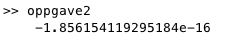
\includegraphics[width=0.4\textwidth]{sections/Exercise2/disp2}
    % \includegraphics[width=0.4\textwidth]{errorplot2}
    \caption{Error - end of beam}
    \label{fig:disp2}
\end{figure}

\begin{figure}[h]
    \centering
    \includegraphics[width=0.8\textwidth]{sections/Exercise2/errorplot2}
    % \includegraphics[width=0.8\textwidth]{errorplot2}
    \caption{Error plot}
    \label{fig:errorplot2}
\end{figure}
 
Plottingen vises i figur \ref{fig:errorplot2}, og man kan se at de to linjene ligger veldig nerme hverandre, som vil si at feilen er svært liten.


% remove after
% \end{document}
\clearpage
%\newpage
% subsection oppgave_2 (end)


\subsection{Oppgave 3} % (fold)
\label{sub:oppgave_3}
% !TEX encoding = UTF-8 Unicode
%\documentclass{article}
%\usepackage{superstyle}

%\begin{document}
Exercise 3!
%\end{document}
\newpage
% subsection oppgave_3 (end)


\subsection{Oppgave 4} % (fold)
\label{sub:oppgave_4}
%!TEX encoding = UTF-8 Unicode
%\documentclass{article}
%\usepackage{listings}
%\usepackage{amsmath}
%\begin{document}
% remove all before

%oppgavetekst

Add a sinusoidal pile to the beam. This means adding a function of form $s(x)=-pg\sin(\frac{\pi}{L}x)$ to the force term $f(x)$. Prove that the solution

\begin{align}
y(x) = \frac{f}{{24EI}}{x^2}({x^2} - 4Lx + 6{L^2}) - \frac{{pgL}}{{EI\pi }}\left( {\frac{{{L^3}}}{{{\pi ^3}}}\sin \frac{\pi }{L} - \frac{{{x^3}}}{6} + \frac{L}{2}{x^2} - \frac{{{L^2}}}{{{\pi ^2}}}x} \right)
\end{align}

satisfies the Euler–Bernoulli beam equation and the clamped-free boundary conditions.

\vspace{5mm}
\textbf{Løsning}

Skal bevise at: 
\begin{align}
\label{ex4}
y(x) &= \frac{f}{{24EI}}{x^2}({x^2} - 4Lx + 6{L^2}) - \frac{{pgL}}{{EI\pi }}\left( {\frac{{{L^3}}}{{{\pi ^3}}}\sin \frac{\pi }{L}x - \frac{{{x^3}}}{6} + \frac{L}{2}{x^2} - \frac{{{L^2}}}{{{\pi ^2}}}x} \right)\nonumber\\ 
EIy(x) &= \frac{f}{{24}}{x^2}({x^2} - 4Lx + 6{L^2}) - \frac{{pgL}}{{\pi }}\left( {\frac{{{L^3}}}{{{\pi ^3}}}\sin \frac{\pi }{L}x - \frac{{{x^3}}}{6} + \frac{L}{2}{x^2} - \frac{{{L^2}}}{{{\pi ^2}}}x} \right)\nonumber\\
%Ganger inn X^2 
EIy(x) &= \frac{f}{{24}}({x^4} - 4Lx^3 + 6{L^2}{x^2}) - \frac{{pgL}}{{\pi }}\left( {\frac{{{L^3}}}{{{\pi ^3}}}\sin \frac{\pi }{L}x - \frac{{{x^3}}}{6} + \frac{L}{2}{x^2} - \frac{{{L^2}}}{{{\pi ^2}}}x} \right)\nonumber\\
%deriverer 1 gang
\intertext{Fjerdederiverer på hver side}
EIy'(x) &= \frac{f}{{24}}(4{x^3} - 12Lx^2 + 12{L^2}x) - \frac{{pgL}}{{\pi }}\left( {\frac{{{L^3}}}{{{\pi ^3}}}\cos (\frac{\pi }{L}x) \cdot \frac{\pi}{L} - \frac{{{3x^2}}}{6} + \frac{2L}{2}x - \frac{{{L^2}}}{{{\pi ^2}}}} \right)\nonumber\\
%deriverer 2 gang
EIy''(x) &= \frac{f}{{24}}(12{x^2} - 24Lx + 12{L^2}) - \frac{{pgL}}{{\pi }}\left( {\frac{{{L^2}}}{{{\pi ^2}}}-\sin (\frac{\pi }{L}x) \cdot \frac{\pi}{L} - x + L } \right)\nonumber\\
%deriverer 3 gang
EIy'''(x) &= \frac{f}{{24}}(24x - 24L) - \frac{{pgL}}{{\pi }}\left( {\frac{{{L}}}{{{\pi}}}-\cos (\frac{\pi }{L}x) \cdot \frac{\pi}{L} - 1 } \right)\nonumber\\
%deriverer 4 gang
EIy''''(x) &= \frac{f}{{24}}(24) - \frac{{pgL}}{{\pi }}\left( {\sin (\frac{\pi }{L}x) \cdot \frac{\pi}{L}  } \right)\nonumber\\
%clean
EIy''''(x) &= \frac{f24}{24} - {pg} \cdot{\sin (\frac{\pi }{L}x) } \nonumber\\
%more clean
EIy''''(x) &= f - {pg} \cdot{\sin (\frac{\pi }{L}x) } \nonumber\\
\end{align}

Vi ser ut ifra resultatet i bevis \ref{ex4} at ligningen er ekvivalent med $s(x)$. 


% remove after
%\end{document}
\newpage
% subsection oppgave_4 (end)


\subsection{Oppgave 5} % (fold)
\label{sub:oppgave_5}
% !TEX encoding = UTF-8 Unicode
% \documentclass{article}
% \usepackage{../../superstyle}
% \usepackage{listings}
% \usepackage{amsmath}
% \begin{document}
% remove all before

%oppgavetekst
Rerun the calculation as in Step 3 for the sinusoidal load. (Be sure to include the weight of the beam itself.) Set p = 100 kg/m and plot your computed solutions against the correct solution. Answer the questions from Step 3, and in addition the following one: Is the error at x = L proportional to $h^2$ as claimed above? You may want to plot the error versus h on a log–log graph to investigate this question. Does the condition number come into play?

\vspace{5mm}
Løsning

\begin{lstlisting}[caption={Oppgave5.m}]
feiltab = zeros(11,1); 
kondtab = zeros(11,1);
h = zeros(11,1);
minst = 100; 
minstTall = 100; 
for(eksp=1:11)
    n=10*(2.^eksp);
    h(eksp) = 2 / n;
    tall1 = lagmatrise(n)\konstantkrefter2(n);
    tall2=korrektutregning2(n); 
    tall3 = tall1(n)-tall2(n); 
    if abs(tall3)<abs(minstTall)
        minst=n; 
        minstTall = tall3; 
    end
    feiltab(eksp)=abs(tall3);
    kondtab(eksp)=condest(lagmatrise(n));
end; 
disp(minst); 
display long; 
disp('Feilene er som folger:'); 
disp(feiltab);
disp('Kondisjonstallene:');
disp(kondtab);
% plot med logaritmiske akser, error vs h^2
loglog(h, h.^2, h, feiltab);
\end{lstlisting}

\begin{lstlisting}[caption={konstantkrefter2.m}]
function [B] = konstantkrefter2(n)
%legger inn rader fra oppgaveteksten. 
%lager høyresiden av matriseligningen. (h^4/EI) * f(x) 
%deler opp bjelken i n lengder med lengde h 
h = 2 / n;        
L=2;
p=100; 
g=-9.81; 
d=480; 
w=0.3;
t=0.03; 
p = 100;
%regner ut kraften f(x) 
kraft = d*w*t*g; 
%definerer E og I som gitt i oppgaven
E = 1.3*10.^(10); 
I = (w*t.^3)/12; 
B = ones(n, 1);
for k=1:n
    xi=k*h; 
    B(k, 1)=g*d*w*t+(p*g*sin(xi*(pi/2)));
end;
B=B*h^4/(E*I);
\end{lstlisting}

\begin{lstlisting}[caption={korrektutregning2.m}]
function [riktig] = korrektutregning2(n)
%deler opp bjelken i n lengder med lengde h 
h = 2 / n;
%regner ut kraften f(x) 
kraft = -9.81*480*0.3*0.03;
%definerer E og I som gitt i oppgaven
E = 1.3*10.^(10); 
I = (0.3*0.03.^3)/12; 
L=2;
p=100; 
g=-9.81;
%initierer matrisen med høyde n
riktig = zeros(n, 1);
for k=1:n
    %hver x er lengden ut i planken vi befinner oss
    x = h * k;
    %formel fra boken, oppgitt i oppgave 4. 
    riktig(k,1)=kraft/(24*E*I)*x.^2*(x.^2-4*L*x+6*(L.^2))
    		+(p*g*L/(E*I*pi))*(L.^3/(pi.^3)*sin(pi/L*x)-(x.^3)/6+(L/2)*x.^2-L.^2/(pi.^2)*x);
end
\end{lstlisting}

\vspace{3mm}

\begin{figure}[h]
\centering
\begin{minipage}{.5\textwidth}
  \centering
  \includegraphics[width=0.5\textwidth]{sections/Exercise5/result5}
    % \includegraphics[width=0.5\textwidth]{result5}
    \caption{Errors - Exercise 5}
    \label{fig:result5}
\end{minipage}%
\begin{minipage}{.5\textwidth}
  \centering
  \includegraphics[width=0.6\textwidth]{sections/Exercise5/cond5}
    % \includegraphics[width=0.6\textwidth]{cond5}
    \caption{Condition numbers - Ex5}
    \label{fig:cond5}
\end{minipage}
\end{figure}

\begin{figure}[h!]
    \centering
    \includegraphics[width=1\textwidth]{sections/Exercise5/loglog5}
    % \includegraphics[width=1\textwidth]{loglog5}
    \caption{Loglog plot - Error(grønn) vs $h^2$}
    \label{fig:loglog5}
\end{figure}

% Answer the questions from Step 3, and in addition the following one: Is the error at x = L proportional to $h^2$ as claimed above? You may want to plot the error versus h on a log–log graph to investigate this question. Does the condition number come into play?

Feilene vises i figur \ref{fig:result5}, i motsetning til hvordan feilen økte med n i oppgave 3, så er den minste feilen her når n = 1280. Før dette vil feilen minke, men etterpå ser det ut som at kondisjonstallet har en større påvirkning, og feilen vil øke proporsjonalt med $h^2$ som man kan se i figur \ref{fig:loglog5}.

% Feilene vises i figur \ref{fig:errors3}, og man kan se at feilen øker når n øker, dette kan man se har en sterk sammenheng med kondisjonstallene som vist i figur \ref{fig:cond3}. Den minste feilen er når k = 1, altså når $n = 10\cdot2^1 = 20$.

% remove after
% \end{document}
\clearpage
%\newpage
% subsection oppgave_5 (end)


\subsection{Oppgave 6} % (fold)
\label{sub:oppgave_6}
% !TEX encoding = UTF-8 Unicode
%\documentclass{article}
%\usepackage{superstyle}

%\begin{document}
%oppgavetekst
Now remove the sinusoidal load and add a 70 kg diver to the beam, balancing on the last 20 cm of the beam. You must add a force per unit length of −g times 70/0.2 kg/m to f (xi ) for all 1.8 ≤ xi ≤ 2, and solve the problem again with the optimal value of n found in Step 5. Plot the solution and find the deflection of the diving board at the free end.

\vspace{5mm}
Løsning

\begin{lstlisting}[caption={Oppgave6regning.m}]
function [B] = Oppgave6Regning(n)
%deler først opp bjelken i n lengder med lengde h 
h = 2 / n;        

%Definerer konstanter. Lengden av planken = 2. g, d, w og t er konstanter i oppgaven. 
L=2;
g=9.81; 
d=480; 
w=0.3;
t=0.03; 

%regner ut kraften f(x) 
kraft = -d*w*t*g; 

%definerer E og I som gitt i oppgaven
E = 1.3*10.^(10); 
I = (w*t.^3)/12; 

%Lager en matrise B med høyde n og bredde 1. 
B = ones(n, 1);

%looper igjennom n
for k=1:n
	%definerer xi for hvert steg ut på brettet
    xi=k*h; 

    %Hvis vi befinner oss på slutten av planken (x mellom 1.8 og 2) er kraften annerledes. (gitt i oppgaven, vekten av stuperen)
    if xi>=1.8
        B(k, 1)=kraft-g*(70/0.2);

    %Hvis ikke er kraften som vanlig:
    else
        B(k, 1)=kraft;
    end
end;

%Til slutt ganger vi hele matrisen med h^4/(E*I)
B=B*h^4/(E*I);
\end{lstlisting}

Vi bruker denne koden til å få den vertikale forskyvningen på slutten av brettet, og lager en graf av brettets vertikale forskyvning:\\

\begin{lstlisting}[caption={Oppgave6.m}]
%Regner matrisen A med alle vertikale forskyvninger langs stupebrettet. Den
%optimale n funnet i forrige oppgave er 1280.
A=Oppgave6Regning(1280); 

%Definerer matrisen B på samme måte som før
B= lagmatrise(1280); 

%Regner ut C, som vil inneholde den vertikale forskyvningen til hvert punkt
%langs stupebrettet. (C=A*Binvers)
C=B\A; 

%Skriver ut den siste vertikale forskyvningen, altså forskyvningen på
%slutten av brettet. 
disp('Vertikal forskyvning på slutten av stupebrettet: '); 
disp(C(1280)); 

%Lager en x-vektor med x-verdier
x=0:(2/1280):(2-2/1280); 

%Lager en graf av x-verdiene og den vertikale forskyvningen
plot(x',C);
\end{lstlisting} 

Den vertikale forskyvningen på slutten av planken er $C(1280)=-0.2034$

\begin{figure}[h]
    \centering
    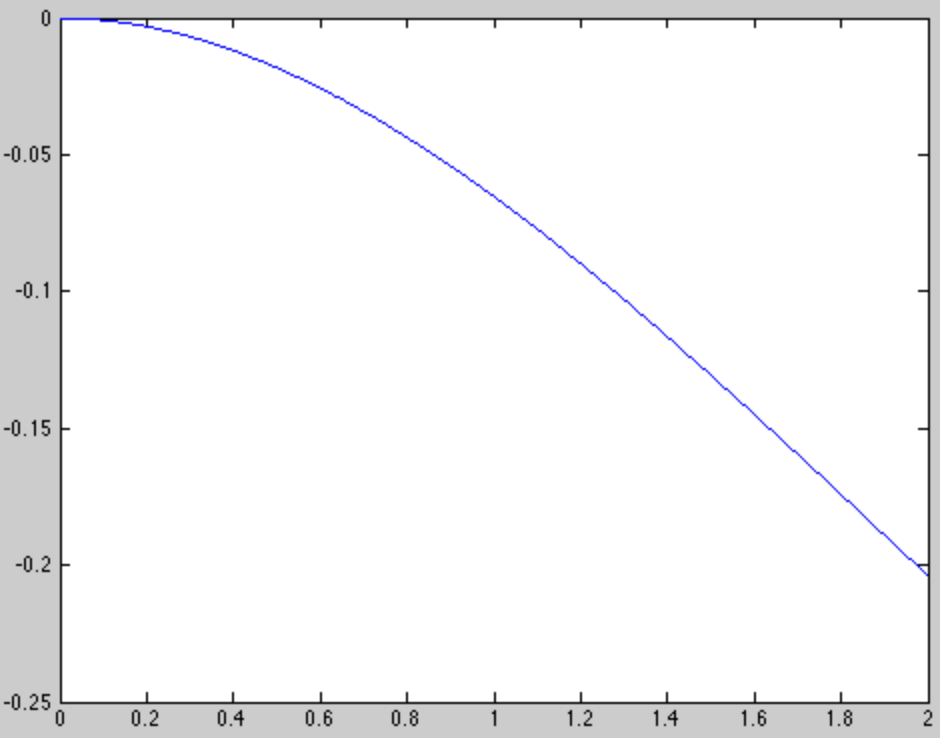
\includegraphics[width=0.8\textwidth]{sections/Exercise6/DiverGraph}
    % \includegraphics[width=0.8\textwidth]{errorplot2}
    \caption{Grafen til stupebrettet påvirket av stuperens vekt}
    \label{fig:divergraph}
\end{figure}

%\end{document}
\clearpage
%\newpage
% subsection oppgave_6 (end)

%section resultater (end)



\section{Konklusjon} % (fold)
\label{sec:konklusjon}
Vi har i denne oppgaven regnet mye på Euler-Bernoulli ligningen for materialers bøyning under påvirkning av ytre- og egenkrefter. Vi har sett at ligningen er svært nøyaktig. Når vi sammenligner den tilnærmede approksimasjonen og den korrekte funksjonen ser vi at feilen i noen tilfeller er lik emach.\ref{fig:errorplot2}\\

En interessant observasjon vi gjorde, var å se hvordan feilen utviklet seg ved stadig minkende h (steglengde). Feilen i diskretiseringen er bevist ved $O(h^2)$. Av dette følger det at feilen, i teorien, vil gå mot 0 når n går mot uendelig $h=\frac{2}{n}$. Dette vil si at jo flere oppdelinger av bjelken vi foretar oss, jo mindre blir feilen gjort i diskretiseringen.\\

Dessverre er det ikke slik i vårt tilfelle. I en perfekt verden, hvor datamaskinene og kalkulatorene kan regne med 100\% nøyaktige tall uten avrundinger, ville dette vært tilfelle. I et av våre tilfeller fant vi ut at feilen var minst ved n=1280. Vi ser av \ref{fig:result5} at feilen synker mot n = 1280, men deretter øker det. Dette vil si at etter n = 1280 har kondisjonstallet en såpass stor påvirkning på utregningene gjort for å finne den vertikale forskyvningen - og derfor stiger feilen. Vi ser at dette stemmer med tabellen over kandisjonstallene \ref{fig:cond5}.\\

Dette er ikke bare tilfelle hvor vi har en sinusformet belastning på bjelken. Det vil være én n for alle typer vekter påført bjelken hvor feilen er minst, og ved å øke n etter dette punktet vil kondisjonstallet øke for mye i forhold til hvor mye vi reduserer h. 


\newpage
% section konklusjon (end)

\newpage
\section{Referanseliste}
\begin{thebibliography}{}
\bibitem{Boka}
  Sauer, T. 
  \emph{Numerical Analysis, Second Edition}
  Pearson Education Limited 2014, Edinburgh Gate, Harlow, England And Associated Companies throughout the world
  
\bibitem{NdogmoEB}
  Ndogmo, J. C. 
  \emph{Equivalence transformations of Euler-Bernoulli equation}.
  School of Mathematics, University of the Witwatersrand, Private Bag 3, Wits 2050, South
Africa

\bibitem{Timoshenko}
  Timoshenko, S.P. 
  \emph{On the transverse vibrations of bars of uniform cross-section}.
  Philosophical Magazine 43 (1922) 125–131
  
\bibitem{Taylor}
   Pauls Online Notes : Calculus II. 
    \emph{http://tutorial.math.lamar.edu/Classes/CalcII/TaylorSeries.aspx} - [25.03.2015]

\end{thebibliography}


\section{Vedlegg} % (fold)
\label{sec:vedlegg}
Her vil du plassere alt som ikke er direkte relevant for rapporten, og som kun vil leses av et lite antall mennesker. Selv de fleste sensorer vil kanskje sjekke kun ett vedlegg for a se at det inneholder det du sier og at det er greit disponert. Hvis man utvikler programvare vil vanligvis utskrift av all kode ligge i vedlegg, mens utdrag fra denne legges inn i bilder eller figurer i teksten, der hvor dette er naturlig. Dette er ogsa stedet for matematisk bevis og liknende (det er forskjell pa matematiske bevis og matematiske teorier og omrader – det siste skal plasseres i teoridelen).
% section vedlegg (end)

\end{document}

